%  !TeX  root  =  user_guide.tex 

\section{Plugin Dxf2Shp Converter}\label{dxf2shape}

% when the revision of a section has been finalized, 
% comment out the following line:
% \updatedisclaimer

Il plugin dxf2shape permette di convertire dati vettoriali dal formato DXF al 
formato shapefile. Vanno impostati i seguenti parametri:

\begin{itemize}
\item \textbf{File DXF in Input}: il percorso del file DXF da convertire
\item \textbf{File di output}: il nome dello shapefile in output
\item \textbf{Tipo di file in output}: il tipo di file in output (scelta tra polilinea, poligono o punto).
\item \textbf{Esporta le etichette di testo}: se selezionata, viene creato uno shapefile di punti. 
La tabella dbf associata conterrà informazioni circa i campi "TESTO" trovati nel file dxf e le stringhe 
di testo stesse.
\end{itemize}

\begin{figure}[ht]
   \centering
   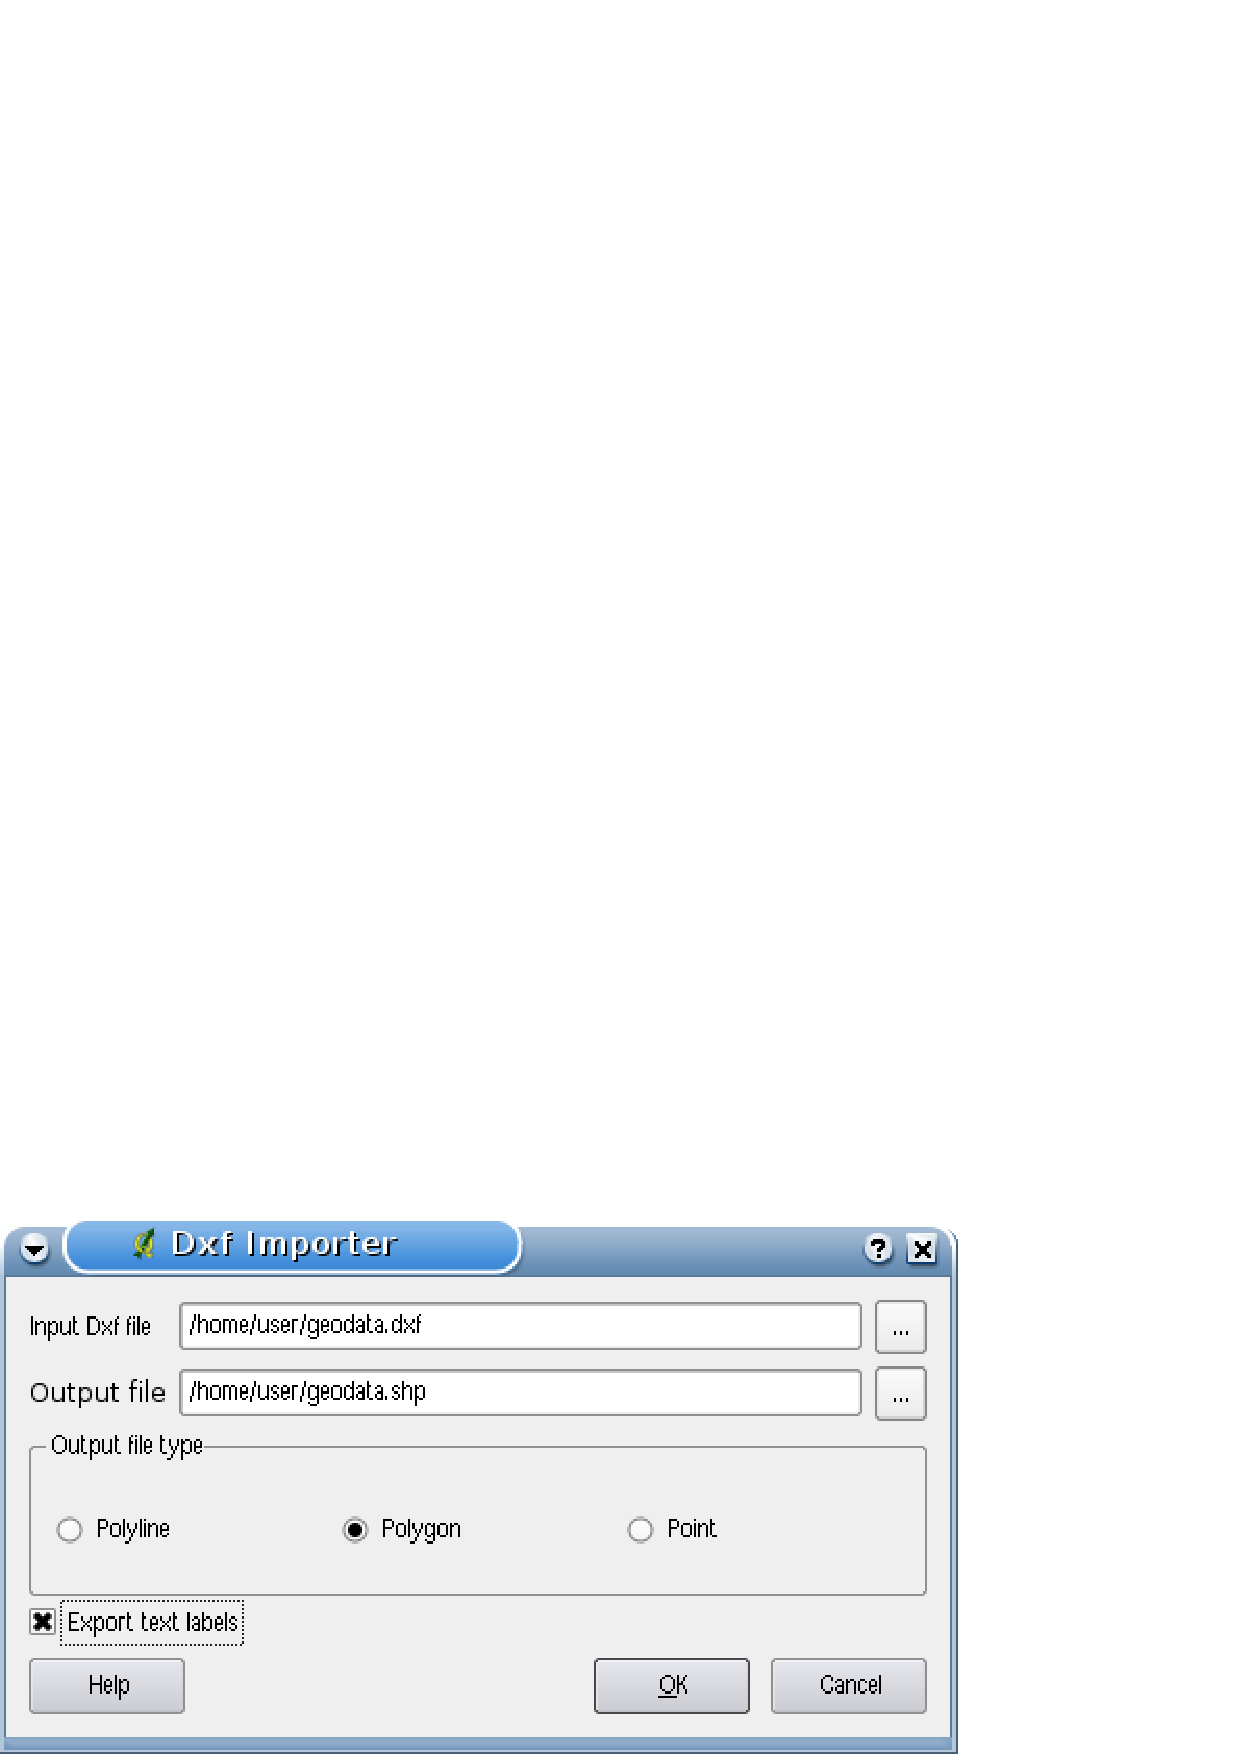
\includegraphics[clip=true, width=9cm]{dxf2shape_dialog}   
   \caption{Plugin Convertitore Dxf2Shape \nixcaption}\label{fig:dxf2shape_dialog}
\end{figure}

\minisec{Utilizzo del plugin}

\begin{enumerate}
  \item Avviare QGIS, attivare il plugin Dxf2Shape dal gestore dei plugin 
  (Sezione \ref{sec:load_core_plugin}) e cliccare sull'icona \toolbtntwo{dxf2shp_converter}{Convertitore Dxf2Shape} 
  che compare nella barra dei plugin. La finestra di dialogo del plugin Dxf2Shape 
  appare come mostrato in Figura \ref{fig:dxf2shape_dialog}.
  \item Caricare il file DXF da convertire, inserire un nome per lo shapefile in output ed il tipo.
  \item Abilitare la casella di controllo \checkbox{Esporta le etichette di testo}, se si vuole
  creare un layer addizionale di punti con le etichette.
  \item Cliccare su \button{Ok}. 
\end{enumerate}

\FloatBarrier